\section{Discovered objects}

Below we list some of the variable objects that have discovered as a result of running the automated pipeline on a fraction of the ULTRACAM archive. All of the objects were noticed after browsing through the light-curves 'by eye'. That is, using a human to visually inspect each light curve one-by-one. This task is made relatively easy in the browser interface and it is possible to inspect at a rate of about 1-2 objects per second. In future, we plan to apply some statistical tests to the data to perform the light curve inspection as a stage of the automated pipeline. Algorithms to perform these sorts of tests are already known and becoming increasingly accurate as more large scale sky surveys launch. We plan to re-use work from one or more of these surveys. References to VVV, LSST, NGTS, Wasp, Astrokit software, etc.

\subsection{Contact binaries}

  \begin{tabular}{l l}
  \hline
  ObjectID & 2013-07-21-run010-163 \\
  Pixel position & (417, 650) \\
  RA, DEC & 19:44:10.3, 40:18:08.1 (J2000) \\
  URL: & \small \url{http://deneb.astro.warwick.ac.uk/phrnaw/sitedev/2013-07-21/run010.html} \\
  Finding chart & 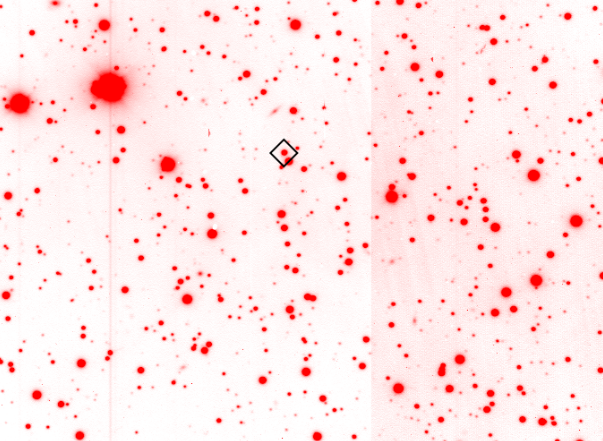
\includegraphics[width=60mm]{images/2013-07-21-run010-163.png} \\
  Light curve & 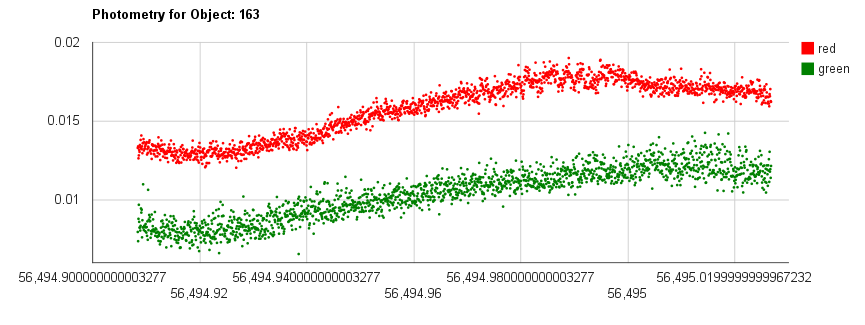
\includegraphics[width=120mm]{images/2013-07-21-run010-163_lightcurve.png} \\
  \hline
  \end{tabular}
  Discussion of this object.

  \begin{tabular}{l l}
  \hline
  ObjectID & 2013-07-21-run010-163 \\
  Pixel position & (417, 650) \\
  RA, DEC & 19:44:10.3, 40:18:08.1 (J2000) \\
  URL: & \small \url{http://deneb.astro.warwick.ac.uk/phrnaw/sitedev/2013-07-21/run010.html} \\
  Finding chart & 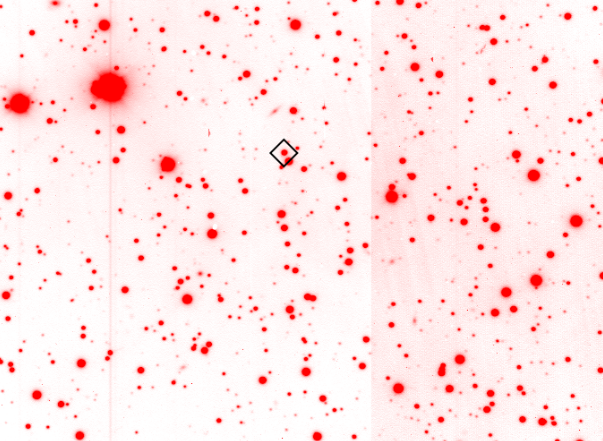
\includegraphics[width=60mm]{images/2013-07-21-run010-163.png} \\
  Light curve & 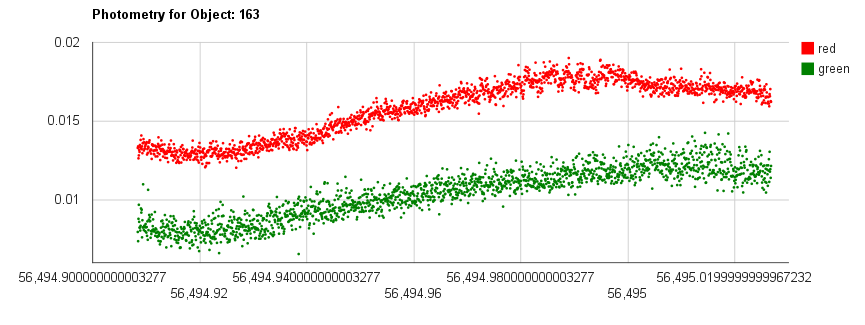
\includegraphics[width=120mm]{images/2013-07-21-run010-163_lightcurve.png} \\
  \hline
  \end{tabular}
  Discussion of this object.

  \begin{tabular}{l l}
  \hline
  ObjectID & 2013-07-21-run010-163 \\
  Pixel position & (417, 650) \\
  RA, DEC & 19:44:10.3, 40:18:08.1 (J2000) \\
  URL: & \small \url{http://deneb.astro.warwick.ac.uk/phrnaw/sitedev/2013-07-21/run010.html} \\
  Finding chart & 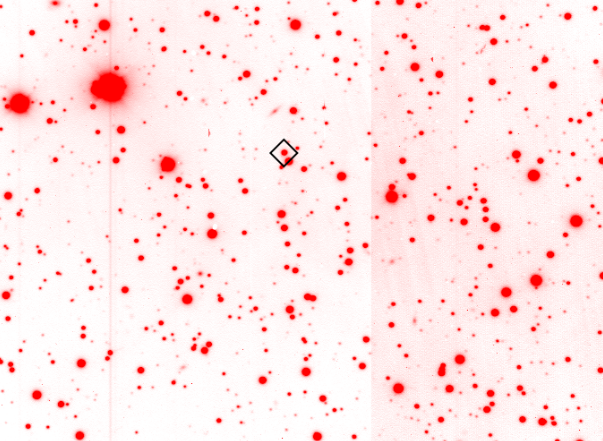
\includegraphics[width=60mm]{images/2013-07-21-run010-163.png} \\
  Light curve & 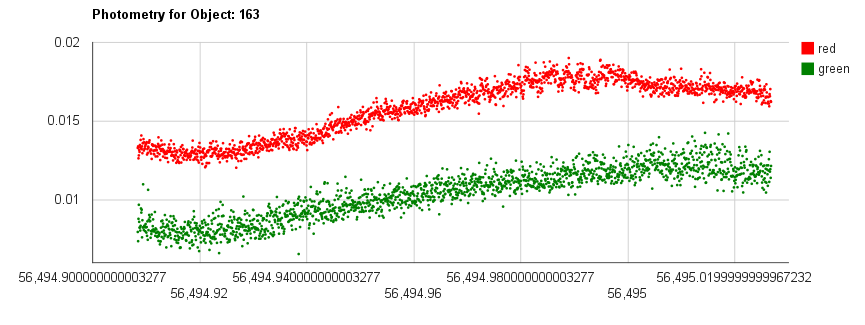
\includegraphics[width=120mm]{images/2013-07-21-run010-163_lightcurve.png} \\
  \hline
  \end{tabular}
  Discussion of this object.

  \begin{tabular}{l l}
  \hline
  ObjectID & 2013-07-21-run010-163 \\
  Pixel position & (417, 650) \\
  RA, DEC & 19:44:10.3, 40:18:08.1 (J2000) \\
  URL: & \small \url{http://deneb.astro.warwick.ac.uk/phrnaw/sitedev/2013-07-21/run010.html} \\
  Finding chart & 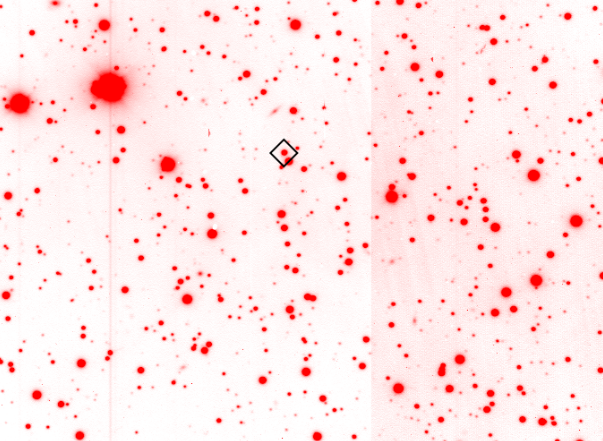
\includegraphics[width=60mm]{images/2013-07-21-run010-163.png} \\
  Light curve & 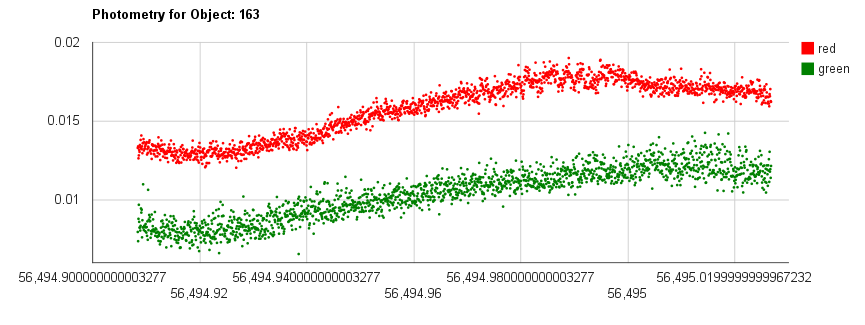
\includegraphics[width=120mm]{images/2013-07-21-run010-163_lightcurve.png} \\
  \hline
  \end{tabular}
  Discussion of this object.

